\section{Durchführung}
\label{sec:Durchführung}
  Es wird die Relaxationszeit $\tau(T)$ von KBr(Sr) mit zwei verschiedenen Heizraten $b_1=\SI{1,9}{\kelvin}/\si{\minute}$ und $b_2=\SI{1,4}{\kelvin}/\si{\minute}=$ bestimmt.

  Der gesamte Versuch wird mit dem unten dargestelltem Aufbau durchgef"uhrt (Abb. \ref{fig:aufbau}).
  Er besteht aus einem Rezipent, in dem sich die Probenkristallplatte zwischen einem Plattenkondensator befindet.
  Der Rezipent wird mit der Vakuumpumpe evakuiert.
  Es kann eine Gleichspannung von bis $\SI{920}{V}$ am Kondensator angelegt werden und mit dem Picoamperemeter der Strom zwischen den Kondensatorplatten gemessen werden.
  Die Probe kann "uber den mit ihr verbundenen K"uhlfinger mit fl"ussigem Stickstoff gek"uhlt werden.
  Durch einen Heizdraht kann die Probe geheizt werden.
  Dabei wird ein Strom von maximal $\SI{3}{\ampere}$ angelegt.
  %Die Probe kann durch eineHeispule mit Heizstrom bis $\SI{3}{A}$ geheizt oder mit fl"ussigem Stickstoff, "uber den mit ihr verbundenen K"uhlfinger, gek"uhlt werden.
  Mit Hilfe eines Thermocouples wird die Temperatur $T$ der Probe gemessen.
  \begin{figure}[H]
    \centering
    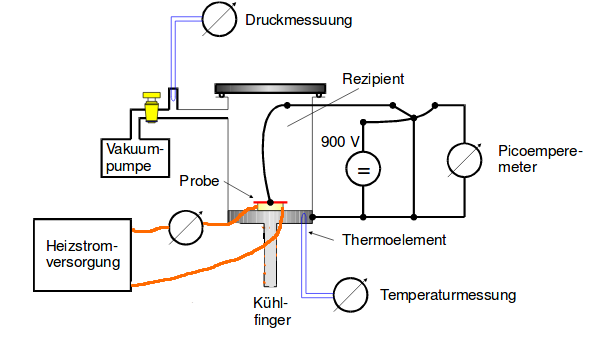
\includegraphics[height=7cm]{bilder/Aufbau.png}
    \caption{Versuchsaufbau bestehend aus dem Rezipenten in dem sich die Probe auf einem Sockel mit K"uhlfinger befindet, eine Vakuumpumpe zum evakuieren, einer Heizstromversorgung und einer Gleichspannungsversorgung zum Anlegen des elektrischen Feldes, sowie dem angeschlossenen Picoampermeter zum Messen des Depolarisationsstroms und einem Temperaturmessger"at \cite{Anleitung}.}
    \label{fig:aufbau}
  \end{figure}
  Der Rezipent ist auf $\SI{0,01}{\milli \bar}$
  evakuiert.
  Zu Beginn der Messung wird die Probe auf die Polarisationstemperatur $T_p=\SI{325}{K}$ gebracht. Am Plattenkondensator wird f"ur $\SI{20}{\minute}$ ein elektrisches Feld $E=U/d$ mit $U=\SI{920}{\volt}$ und $d=\SI{3}{\milli \meter}$ angelegt, w"ahrenddessen wird die Polarisationstemperatur $T_p$ beibehalten.
  Dann wird der K"uhlfinger mit fl"ussigem Stickstoff umgeben und die Probe so auf $T_0=\SI{217}{\kelvin}$ abgek"uhlt.
  Danach wird der Kondensator f"ur $\SI{10}{\minute}$ geerdet, um "ubersch"ussige Ladung abflie"sen zu lassen.

  Nun wird mit der eigentlichen Messung begonnen, bei der die Probe mit einer Heizrate von $b_1=\SI{1,8}{\kelvin}/\si{\minute}$ geheizt wird und von $T=T_0$ bis $T=\SI{333}{\kelvin}$ jede Minute der Depolarisationsstrom $i(T)$ und zugeh"orige Probentemperatur $T$ notiert werden.
  Diese Schritte werden bei demselben Probenkristall f"ur eine zweite Heizrate von $b_2=\SI{1,4}{\kelvin}/\si{\minute}$ wiederholt.
